\subsection{UniProt}
\label{uniprotdb}

\subsubsection{Introduction}
It is important to restate the goal of the \xmlpipedb~project before understanding 
the important role \emph{uniprotdb} played in the project; To create a reusable tool set 
that given genomic sequencing data for an organism in XML and a schema for that 
XML document could output a working \genmapp~gene database for that organism.  During
the beginning phases of the project, there was only one project, \xmlpipedb, and it
made use of the schema provided by the UniProt Consortium~\cite{uniprotWeb}.  However,
it soon became evident that the project could be designed in a manner that would 
allow a wider audience the use of our tool.  The first phase was \emph{xsd2db} (Section~\ref{xsd2db})  which allowed for the use of any schema
to create the necessary JAXB objects and hibernate mappings.  However, we still
needed to create a tool specific for the UniProt XML and XSD.  At that point, \emph{uniprotdb}
was born.  

\subsubsection{Design}
Before the project was split into a variety of subprojects, \xmlpipedb~offered
the ability to use the UniProt schema and create the necessary JAXB objects
and \hibernate~mappings.  It created these files in default directories that 
are called out in the \hyperjaxb2~template project~\cite{hyperjaxb}.  Customizations were used in order to get \xmlpipedb~to work properly, but we hoped 
to further understand how to use \hyperjaxb2~customizations to overcome these issues.  
Section~\ref{uniprotImplementation} discusses in further detail the \hyperjaxb2~customizations that were needed for \xmlpipedb~to function.  

Once it was determined that we wanted to allow groups outside the Bioinformatics community the 
use of our tool, \emph{uniprotdb} became its own subproject.  \emph{uniprotdb}
would be created from the output of \emph{xsd2db}.  It would contain the UniProt schema,
customized external binding file, 
SQL DDL file that corresponds to the schema, the JAXB objects, and the \hibernate~mappings.  
The layout 
shown in Figure~\ref{fig:uniprotLayout} was what we hoped uniprotdb would look like.  

\begin{figure}[htp]
\centering
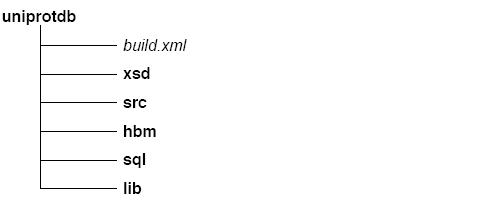
\includegraphics[scale=1.0]{Images/uniprotLayout.jpg}
\caption{\small \sl The uniprotdb layout.} 
\label{fig:uniprotLayout}
\end{figure}

The build file would have the following capabilities:
\begin{itemize}
  \item \textit{compile} compiles the JAXB objects located within the src directory with help from any necessary jars located in the lib directory

  \item \textit{jar} compile and create a jar file containing the class files derived from the src directory and the hibernate mappings located within the hbm directory
  
  \item \textit{clean} eliminates all the products of a previous build.  
\end{itemize}
The jar file created as a result of a build would later be used in the gmbuilder 
subproject, thoroughly outlined in Section~\ref{gmbuilder}.  Once uniprotdb was
created, we would have been one step closer to creating a \genmapp~usable, gene 
database.  

\subsubsection{Implementation}
\label{uniprotImplementation}
% discuss phases of the post processor and the failed usage of hibernate bindings
The work we did on the original \xmlpipedb~project set the stage for the creation of
uniprotdb.  
The work on the original \xmlpipedb~project brought us to a point where we were able to load
the SQL DDL file that was produced from the UniProt schema.  In addition, we were able to 
import the JAXB objects into the database.  Before this point was reached though, we had to
overcome three issues with the hyperjaxb2 and the UniProt schema.  The issues that slowed our 
progress with \xmlpipedb~were:
\begin{itemize}
   \item PostgreSQL doesn�t like attributes whose name is ``end'' (see LocationType in UniProt XSD)
   
   \item String types default to a maximum length of 255 (varchar(255)), but some strings in the UniProt XML files exceed this length
   
   \item Hyperjaxb2's handling of the xsd:union tag doesn�t seem to work properly, resulting in MappingExceptions when attempting to load an XML file
\end{itemize}

The solution at the time was to manually edit the generated files.  The
SQL DDL file that corresponds to the UniProt schema had a need for multiple edits.  The
first was to change``end'' to 
``endPosition.''  This solved the problem with keyword ``end'' in PostgreSQL.  
The second edit was to change ``varchar(255)'' to just ``varchar.''  This solved any issues with
there being a maximum length for strings within a UniProt XML file.  

Since we changed the SQL DDL column named ``end'' to 
``endPosition,'' the same change needed to be made to the corresponding hibernate mapping file.  
This edit took place within LocationType.hbm.xml.    
Lastly, CitationType.hbm.xml needed to be manually edited due to the xsd:union 
tag being an issue with hyperjaxb2.  The ``Date'' field of CitationType allowed for any form of Date,
whereas the best solution was to only allow strings.  So CitationType.hbm.xml was updated to only allow
strings for Citation Dates.  Once all these issues were resolved, the import of a UniProt XML file
into the database was no longer a problem.  

At about the time \xmlpipedb~was beginning to show promise, the decision was made to split the \xmlpipedb~project into a group of smaller projects that would allow for groups outside the Bioinformatics
community to use our tool.  Hence, uniprotdb was supposed to be a subproject specific to the 
UniProt schema.  Rather than forcing the user have to manually edit the output of xsd2db due to the issues
above, we looked
at the use of a customizable binding file within hyperjaxb2.  Custom binding files would allow for changes
to a schema and its generated files without any extra work required by the user.  The use of custom bindings 
files were looked at for a few weeks before it was stopped due to complexity and time constraints.  Refer to 
Section~\ref{uniprotImprovements} for further detail regarding custom bindings files.  

Once it was determined that custom bindings would not be used, we needed an alternative method to the 
editing of the generated files from xsd2db.  We decided to develop a post processor.  The post processor
would reside within the uniprotdb project under a new directory named tools.  Within the tools directory
would be a build file, a README file, and the necessary source code to do the post processing.  The build
file had the ability to compile the source code and eliminate all the products of a previous build.  

The post processor had the ability to be run via command line with options to specify the locations of the files
to be edited or with the use of a graphical user interface (GUI).  With the GUI, there are two windows shown
for each file.  The first window asks for the user to locate the file to post process.  It is shown in 
Figure~\ref{fig:locateFile}.  
\begin{figure}[htp]
\centering
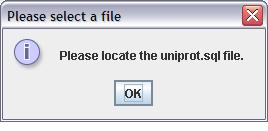
\includegraphics[scale=1.0]{Images/locateFile.jpg}
\caption{\small \sl The locate file dialog.} 
\label{fig:locateFile}
\end{figure}
Once the user hits the OK button, a second window appears.  The second window is a file dialog for the 
user to use as a navigator for the file to be processed.  It is shown in Figure~\ref{fig:chooseFile}.  
\begin{figure}[htp]
\centering
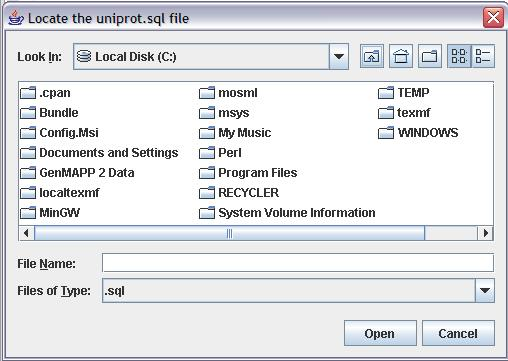
\includegraphics[scale=0.80]{Images/chooseFile.jpg}
\caption{\small \sl The choose file dialog.} 
\label{fig:chooseFile}
\end{figure}
After the last file is processed, the window in Figure~\ref{fig:success} appears to let the user know that 
the operation was successful.  
\begin{figure}[htp]
\centering
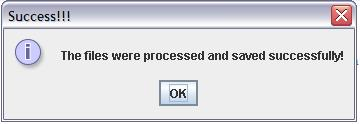
\includegraphics[scale=1.0]{Images/success.jpg}
\caption{\small \sl The success window.} 
\label{fig:success}
\end{figure}

Further testing resulted in the finding of more bugs with the ``Date'' field
in the schema.  As a result, the post processor needed to be updated to
process two more java classes.  CitationType.java and CitationTypeImpl.java both
needed post processing to make sure that the ``Date'' field used by the
JAXB objects would only return a object of type string.  With the addition
of two more files being post processed, the decision was made to no longer
make the command line version of the post processor available.  We felt
that the user should not be burdened with having to fill in the absolute
path for a total of five files.  

\subsubsection{Future Work and Improvements}
\label{uniprotImprovements}
The only visible improvement to uniprotdb would be to use a custom mapping file rather than a post 
processing tool.  The custom mapping file would be used with xsd2db and the UniProt schema and would
allow custom mappings to be generated for classes and fields by annotating the schema.  This would no 
longer make a post processor needed.  

The future of uniprotdb is up in the air.  Only a small subset of the total UniProt XML files available 
have been imported into a database with gmbuilder.  
This means that more post processing may be needed because all the post processing
needs may have not been discovered.  As testing continues, the Bioinformatics community will need
to feel free to report any bugs and errors.  In addition, a new UniProt schema could become
available resulting in more post processing.  As a result, it will be the responsibility of 
this group of developers to keep track of the ever changing Bioinformatics landscape.  

\subsubsection{Conclusion}
uniprotdb is important in order to reach our goal of creating a gene database that can be used by
the \genmapp~application.  xsd2db creates the necessary JAXB objects and hibernate mappings corresponding
to the UniProt schema.  The uniprotdb post processing tool also appears to work with the current
UniProt schema.  However, a much cleaner implementation would make use of a custom bindings file.  Future
implementations of uniprotdb should look at the process of creating custom bindings file again.  
It must be noted though, as simple as uniprotdb is, it is crucial for gmbuilder application 
to function properly.  
